%\hypertarget{___gatsby}{}
%\hypertarget{gatsby-focus-wrapper}{}
%\href{https://mukulrathi.com/}{}
%
%MUKUL RATHI
%
%\href{https://mukulrathi.com/about-me}{}
%
%About Me
%
%\href{https://mukulrathi.com/blog}{}
%
%Blog
%
%\hypertarget{creating-the-bolt-compiler-part-8}{%
%\subsection{Creating the Bolt Compiler: Part
%8}\label{creating-the-bolt-compiler-part-8}}

\hypertarget{top-of-page}{%
\chapter{A Complete Guide to LLVM for Programming Language
Creators}\label{top-of-page}}

December 24, 2020
%
%\hypertarget{december-24-2020}{%
%\subsection{December 24, 2020}\label{december-24-2020}}
%
%\hypertarget{min-read}{%
%\subsection{12 min read}\label{min-read}}

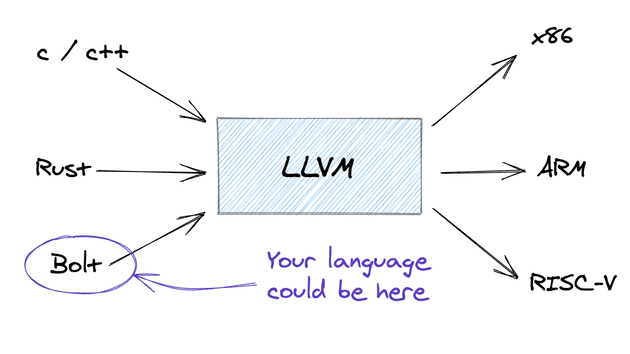
\includegraphics[width=\linewidth]{08_files/llvm.png}

%\hypertarget{series-creating-the-bolt-compiler}{%
%\section{Series: Creating the Bolt
%Compiler}\label{series-creating-the-bolt-compiler}}
%
%\begin{itemize}
%\item
%  { Part 1:
%  }\href{https://mukulrathi.com/create-your-own-programming-language/intro-to-compiler/}{How
%  I wrote my own "proper" programming language}
%\item
%  { Part 2:
%  }\href{https://mukulrathi.com/create-your-own-programming-language/compiler-engineering-structure/}{So
%  how do you structure a compiler project?}
%\item
%  { Part 3:
%  }\href{https://mukulrathi.com/create-your-own-programming-language/parsing-ocamllex-menhir/}{Writing
%  a Lexer and Parser using OCamllex and Menhir}
%\item
%  { Part 4:
%  }\href{https://mukulrathi.com/create-your-own-programming-language/intro-to-type-checking/}{An
%  accessible introduction to type theory and implementing a
%  type-checker}
%\item
%  { Part 5:
%  }\href{https://mukulrathi.com/create-your-own-programming-language/data-race-dataflow-analysis/}{A
%  tutorial on liveness and alias dataflow analysis}
%\item
%  { Part 6:
%  }\href{https://mukulrathi.com/create-your-own-programming-language/lower-language-constructs-to-llvm/}{Desugaring
%  - taking our high-level language and simplifying it!}
%\item
%  { Part 7:
%  }\href{https://mukulrathi.com/create-your-own-programming-language/protobuf-ocaml-cpp-tutorial/}{A
%  Protobuf tutorial for OCaml and C++}
%\item
%  \textbf{Part 8: A Complete Guide to LLVM for Programming Language
%  Creators}
%\item
%  { Part 9:
%  }\href{https://mukulrathi.com/create-your-own-programming-language/concurrency-runtime-language-tutorial/}{Implementing
%  Concurrency and our Runtime Library}
%\item
%  { Part 10:
%  }\href{https://mukulrathi.com/create-your-own-programming-language/generics-parametric-polymorphism/}{Generics
%  - adding polymorphism to Bolt}
%\item
%  { Part 11:
%  }\href{https://mukulrathi.com/create-your-own-programming-language/inheritance-method-overriding-vtable/}{Adding
%  Inheritance and Method Overriding to Our Language}
%\end{itemize}
%
%\begin{center}\rule{0.5\linewidth}{0.5pt}\end{center}

\textbf{Update}: this post has now taken off on
\href{https://news.ycombinator.com/item?id=25539797}{Hacker News} and
\href{https://www.reddit.com/r/programming/comments/kjjijf/a_complete_guide_to_llvm_for_programming_language/}{Reddit}.
Thank you all!

\hypertarget{whos-this-tutorial-for}{%
\section{\texorpdfstring{\protect\hyperlink{whos-this-tutorial-for}{}Who's
this tutorial
for?}{Who's this tutorial for?}}\label{whos-this-tutorial-for}}

This series of compiler tutorials is for people who don't just want to
create a \emph{toy} language. You want objects. You want polymorphism.
You want concurrency. You want garbage collection. Wait you don't want
GC? Okay, no worries, we won't do that :P

If you've just joined the series at this stage, here's a quick recap.
We're designing a Java-esque concurrent object-oriented programming
language \emph{Bolt}. We've gone through the compiler frontend, where
we've done the parsing, type-checking and dataflow analysis. We've
\href{https://mukulrathi.com/create-your-own-programming-language/lower-language-constructs-to-llvm/}{desugared
our language to get it ready for LLVM} - the main takeaway is that
objects have been desugared to structs, and their methods desugared to
functions.

Learn about LLVM and you'll be the envy of your friends. Rust uses LLVM
for its backend, so it must be cool. You'll beat them on all those
performance benchmarks, without having to hand-optimise your code or
write machine assembly code. Shhhh, I won't tell them.

\hypertarget{just-give-me-the-code}{%
\section{\texorpdfstring{\protect\hyperlink{just-give-me-the-code}{}Just
give me the
code!}{Just give me the code!}}\label{just-give-me-the-code}}

All the code can be found in the
\href{https://github.com/mukul-rathi/bolt}{Bolt compiler repository}.

The C++ class definitions for our desugared representation (we call this
\emph{Bolt IR}) can be found in
\href{https://github.com/mukul-rathi/bolt/tree/master/src/llvm-backend/deserialise_ir}{deserialise\_ir}
folder. The code for this post (the LLVM IR generation) can be found in
the
\href{https://github.com/mukul-rathi/bolt/tree/master/src/llvm-backend/llvm_ir_codegen}{llvm\_ir\_codegen}
folder. The repo uses the Visitor design pattern and ample use of
\texttt{std::unique\_ptr} to make memory management easier.

To cut through the boilerplate, to find out how to generate LLVM IR for
a particular language expression, search for the
\texttt{IRCodegenVisitor::codegen} method that takes in the
corresponding \texttt{ExprIR} object. e.g. for if-else statements:

%Copy

\begin{lstlisting}[language=C++]
Value *IRCodegenVisitor::codegen(const ExprIfElseIR &expr) {
      ...
 // this is the LLVM IR generation
}
\end{lstlisting}

\hypertarget{understanding-llvm-ir}{%
\section{\texorpdfstring{\protect\hyperlink{understanding-llvm-ir}{}Understanding
LLVM IR}{Understanding LLVM IR}}\label{understanding-llvm-ir}}

LLVM sits in the \textbf{middle-end} of our compiler, \emph{after} we've
desugared our language features, but \emph{before} the backends that
target specific machine architectures (x86, ARM etc.)

LLVM's IR is pretty low-level, it can't contain language features
present in some languages but not others (e.g. classes are present in
C++ but not C). If you've come across instruction sets before, LLVM IR
is a
\href{https://en.wikipedia.org/wiki/Reduced_instruction_set_computer\#:~:text=A\%20reduced\%20instruction\%20set\%20computer,instruction\%20set\%20computer\%20(CISC).}{RISC}
instruction set.

The upshot of it is that LLVM IR looks like a more \emph{readable} form
of assembly. As LLVM IR is \textbf{machine independent}, we don't need
to worry about the number of registers, size of datatypes, calling
conventions or other machine-specific details.

So instead of a fixed number of physical registers, in LLVM IR we have
an unlimited set of \emph{virtual} registers (labelled \texttt{\%0},
\texttt{\%1}, \texttt{\%2}, \texttt{\%3}\ldots{} we can write and read
from. It's the backend's job to map from virtual to physical registers.

And rather than allocating specific sizes of datatypes, we retain
\textbf{types} in LLVM IR. Again, the backend will take this type
information and map it to the size of the datatype. LLVM has types for
different sizes of \texttt{int}s and floats, e.g. \texttt{int32},
\texttt{int8}, \texttt{int1} etc. It also has derived types: like
\textbf{pointer} types, \textbf{array} types, \textbf{struct} types,
\textbf{function} types. To find out more, check out the
\href{https://llvm.org/doxygen/classllvm_1_1Type.html}{Type}
documentation.

Now, built into LLVM are a set of optimisations we can run over the LLVM
IR e.g.
\href{https://en.wikipedia.org/wiki/Dead_code_elimination}{dead-code
elimination},
\href{https://en.wikipedia.org/wiki/Inline_expansion}{function
inlining},
\href{https://cran.r-project.org/web/packages/rco/vignettes/opt-common-subexpr.html}{common
subexpression elimination} etc. The details of these algorithms are
irrelevant: LLVM implements them for us.

Our side of the bargain is that we write LLVM IR in
\href{https://en.wikipedia.org/wiki/Static_single_assignment_form}{Static
Single Assignment (SSA) form}, as SSA form makes life easier for
optimisation writers. SSA form sounds fancy, but it just means we define
variables before use and assign to variables \textbf{only once}. In SSA
form, we cannot reassign to a variable, e.g. \texttt{x\ =\ x+1}; instead
we assign to a fresh variable each time (\texttt{x2\ =\ x1\ +\ 1}).

So in short: LLVM IR looks like assembly with \textbf{types}, minus the
messy machine-specific details. LLVM IR must be in SSA form, which makes
it easier to optimise. Let's look at an example!

\hypertarget{an-example-factorial}{%
\subsection{\texorpdfstring{\protect\hyperlink{an-example-factorial}{}An
example: Factorial}{An example: Factorial}}\label{an-example-factorial}}

Let's look at a simple factorial function in our language Bolt:



%Copy

\begin{lstlisting}[caption={{factorial.bolt}}]
function int factorial(int n){
  if (n==0) {    1  }
  else{    n * factorial(n - 1)  }
}
\end{lstlisting}

The corresponding LLVM IR is as follows:



%Copy

\begin{lstlisting}[caption={{factorial.ll}},language=llvm]
define i32 @factorial(i32) {
entry:
  %eq = icmp eq i32 %0, 0   // n == 0
  br i1 %eq, label %then, label %else

then:                                             ; preds = %entry
  br label %ifcont

else:                                             ; preds = %entry
  %sub = sub i32 %0, 1   // n - 1
  %2 = call i32 @factorial(i32 %sub) // factorial(n-1)
  %mult = mul i32 %0, %2  // n * factorial(n-1)
  br label %ifcont

ifcont:                                           ; preds = %else, %then
  %iftmp = phi i32 [ 1, %then ], [ %mult, %else ]
  ret i32 %iftmp
}
\end{lstlisting}

Note the \texttt{.ll} extension is for \textbf{human-readable} LLVM IR
output. There's also \texttt{.bc} for bit-code, a more compact machine
representation of LLVM IR.

We can walk through this IR in 4 levels of detail:

\hypertarget{at-the-instruction-level}{%
\paragraph{\texorpdfstring{\protect\hyperlink{at-the-instruction-level}{}At
the Instruction
Level:}{At the Instruction Level:}}\label{at-the-instruction-level}}

Notice how LLVM IR contains assembly instructions like \texttt{br} and
\texttt{icmp}, but abstracts the machine-specific messy details of
function calling conventions with a single \texttt{call} instruction.

{
\href{https://mukulrathi.com/static/f987ee45552570ad7aa513f6d3fc19a7/565cc/factorial-instructions.png}{{}
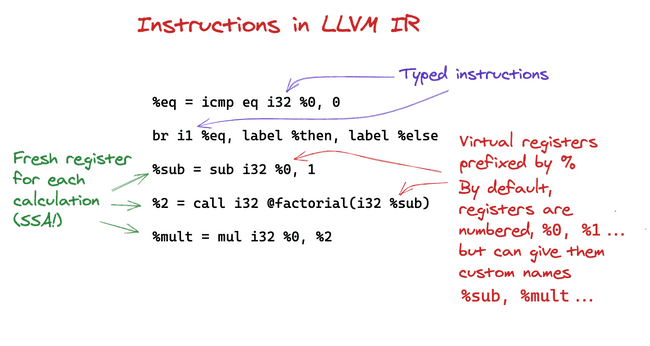
\includegraphics[width=\linewidth]{08_files/factorial-instructions.png}} }

\hypertarget{at-the-control-flow-graph-level}{%
\paragraph{\texorpdfstring{\protect\hyperlink{at-the-control-flow-graph-level}{}At
the Control Flow Graph
Level:}{At the Control Flow Graph Level:}}\label{at-the-control-flow-graph-level}}

If we take a step back, you can see the IR defines the \textbf{control
flow graph} of the program. IR instructions are grouped into labeled
\textbf{basic blocks}, and the \texttt{preds} labels for each block
represent incoming edges to that block. e.g. the \texttt{ifcont} basic
block has predecessors \texttt{then} and \texttt{else}:

At this point, I'm going to assume you have come across Control Flow
Graphs and basic blocks. We introduced Control Flow Graphs in a previous
post in the series, where we used them to perform different dataflow
analyses on the program. I'd recommend you go and check the
\href{http://mukulrathi.co.uk/create-your-own-programming-language/data-race-dataflow-analysis/\#control-flow-graph}{CFG
section of that dataflow analysis post} now. I'll wait here :)

{
\href{https://mukulrathi.com/static/6a6edf6d916150ea4de92c0fc1a68e1a/11864/factorial-cfg.png}{{}
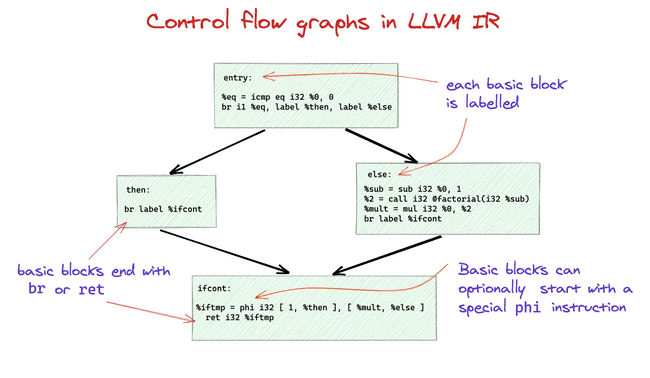
\includegraphics[width=\linewidth]{08_files/factorial-cfg.png}} }

The \texttt{phi} instruction represents \textbf{conditional assignment}:
assigning different values depending on which preceding basic block
we've just come from. It is of the form
\texttt{phi\ type\ {[}val1,\ predecessor1{]},\ {[}val2,\ predecessor2{]},\ ...}
In the example above, we set \texttt{\%iftmp} to 1 if we've come from
the \texttt{then} block, and \texttt{\%mult} if we've come from the
\texttt{else} block. Phi nodes must be at the \textbf{start} of a block,
and include one entry for each predecessor.

\hypertarget{at-the-function-level}{%
\paragraph{\texorpdfstring{\protect\hyperlink{at-the-function-level}{}At
the Function
Level:}{At the Function Level:}}\label{at-the-function-level}}

Taking another step back, the overall structure of a function in LLVM IR
is as follows:

{
\href{https://mukulrathi.com/static/c80bbba94459a0ac84429c53299823b2/b2b2c/factorial-fn.png}{{}
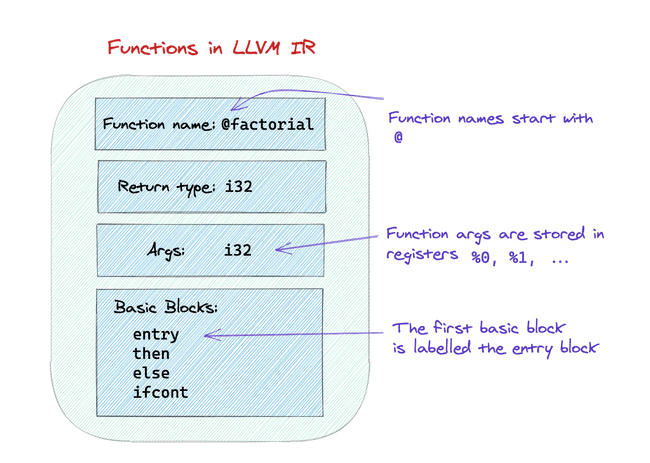
\includegraphics[width=\linewidth]{08_files/factorial-fn.png}} }

\hypertarget{at-the-module-level}{%
\paragraph{\texorpdfstring{\protect\hyperlink{at-the-module-level}{}At
the Module Level:}{At the Module Level:}}\label{at-the-module-level}}

An LLVM \textbf{module} contains all the information associated with a
program file. (For multi-file programs, we'd link together their
corresponding modules.)

{
\href{https://mukulrathi.com/static/e21edb9623d8fb7bc23f57db23b93cf8/cad61/module.png}{{}
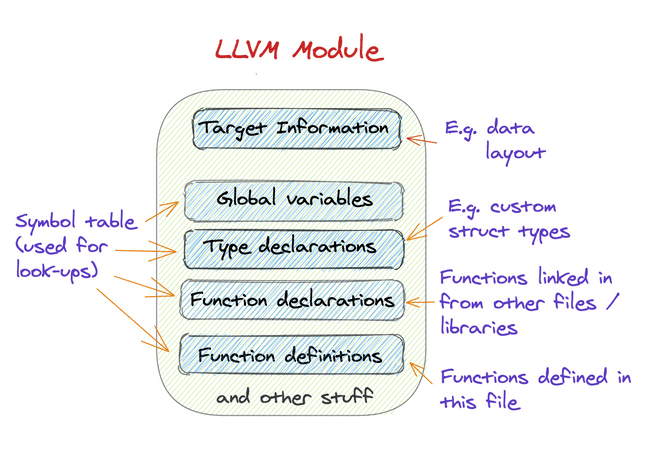
\includegraphics[width=\linewidth]{08_files/module.png}} }

Our \texttt{factorial} function is just one function definition in our
module. If we want to execute the program, e.g. to compute
\texttt{factorial(10)} we need to define a \texttt{main} function, which
will be the entrypoint for our program's execution. The \texttt{main}
function's signature is a hangover from C (we return 0 to indicate
successful execution):



%Copy

\begin{lstlisting}[caption={{example\_program.c}},language=C]
// a C main function
int main(){
  factorial(10);
  return 0;
}
\end{lstlisting}

We specify that we want to compile for an Intel Macbook Pro in the
module target info:



%Copy

\begin{lstlisting}[caption={{example\_module.ll}},language=llvm]
source_filename = "Module"
target triple = "x86_64-apple-darwin18.7.0"
...
define i32 @factorial(i32) {
  ...
}
define i32 @main() {
entry:
  %0 = call i32 @factorial(i32 10)
  ret i32 0
}
\end{lstlisting}

\hypertarget{the-llvm-api-key-concepts}{%
\section{\texorpdfstring{\protect\hyperlink{the-llvm-api-key-concepts}{}The
LLVM API: Key
Concepts}{The LLVM API: Key Concepts}}\label{the-llvm-api-key-concepts}}

Now we've got the basics of LLVM IR down, let's introduce the LLVM API.
We'll go through the key concepts, then introduce more of the API as we
explore LLVM IR further.

LLVM defines a whole host of classes that map to the concepts we've
talked about.

\begin{itemize}
\tightlist
\item
  \texttt{Value}
\item
  \texttt{Module}
\item
  \texttt{Type}
\item
  \texttt{Function}
\item
  \texttt{BasicBlock}
\item
  \texttt{BranchInst} \ldots{}
\end{itemize}

These are all in the namespace \texttt{llvm}. In the Bolt repo, I chose
to make this namespacing explicit by referring to them as
\texttt{llvm::Value}, \texttt{llvm::Module} etc.)

Most of the LLVM API is quite mechanical. Now you've seen the diagrams
that define modules, functions and basic blocks, the relationship
between their corresponding classes in the API falls out nicely. You can
query a \texttt{Module} object to get a list of its \texttt{Function}
objects, and query a \texttt{Function} to get the list of its
\texttt{BasicBlock}s, and the other way round: you can query a
\texttt{BasicBlock} to get its parent \texttt{Function} object.

\texttt{Value} is the base class for any value computed by the program.
This could be a function (\texttt{Function} subclasses \texttt{Value}),
a basic block (\texttt{BasicBlock} also subclasses \texttt{Value}), an
instruction, or the result of an intermediate computation.

Each of the expression \texttt{codegen} methods returns a
\texttt{Value\ *}: the result of executing that expression. You can
think of these \texttt{codegen} methods as generating the IR for that
expression and the \texttt{Value\ *} representing the virtual register
containing the expression's result.

%{
%\href{https://github.com/mukul-rathi/bolt/blob/master/src/llvm-backend/llvm_ir_codegen/ir_codegen_visitor.h\#L64-L84}{ir\_codegen\_visitor.h}}
%
%Copy

\begin{lstlisting}[caption={ir\_codegen\_visitor.h},language=C++]
virtual Value *codegen(const ExprIntegerIR &expr) override;
virtual Value *codegen(const ExprBooleanIR &expr) override;
virtual Value *codegen(const ExprIdentifierIR &expr) override;
virtual Value *codegen(const ExprConstructorIR &expr) override;
virtual Value *codegen(const ExprLetIR &expr) override;
virtual Value *codegen(const ExprAssignIR &expr) override;
\end{lstlisting}

How do we generate the IR for these expressions? We create a
\textbf{unique} \texttt{Context} object to tie our whole code generation
together. We use this \texttt{Context} to get access to core LLVM data
structures e.g LLVM modules and \texttt{IRBuilder} objects.

We'll use the context to create just one module, which we'll
imaginatively name \texttt{"Module"}.

%{
%\href{https://github.com/mukul-rathi/bolt/blob/master/src/llvm-backend/llvm_ir_codegen/ir_codegen_visitor.cc\#L17-L19}{ir\_codegen\_visitor.cc}}
%
%Copy

\begin{lstlisting}[language=C++,caption={ir\_codegen\_visitor.cc}]
context = make_unique<LLVMContext>();
builder = std::unique_ptr<IRBuilder<>>(new IRBuilder<>(*context));
module = make_unique<Module>("Module", *context);
\end{lstlisting}

\hypertarget{irbuilder}{%
\subsection{\texorpdfstring{\protect\hyperlink{irbuilder}{}IRBuilder}{IRBuilder}}\label{irbuilder}}

We use the \texttt{IRBuilder} object to incrementally build up our IR.
It is intuitively the equivalent of a file pointer when reading/writing
a file - it carries around \emph{implicit} state, e.g. the last
instruction added, the basic block of that instruction etc. Like moving
around a file pointer, you can set the \texttt{builder} object to insert
instructions at the end of a particular Basic Block with the
\texttt{SetInsertPoint(BasicBlock\ *TheBB)} method. Likewise you can get
the current basic block with \texttt{GetInsertBlock()}.

The builder object has \texttt{Create\_\_\_()} methods for each of the
IR instructions. e.g. \texttt{CreateLoad} for a \texttt{load}
instruction , \texttt{CreateSub}, \texttt{CreateFSub} for integer and
floating point \texttt{sub} instructions respectively etc. Some
\texttt{Create\_\_()} instructions take an optional \texttt{Twine}
argument: this is used to give the result's register a custom name. e.g.
\texttt{iftmp} is the twine for the following instruction:

\texttt{\%iftmp\ =\ phi\ i32\ {[}\ 1,\ \%then\ {]},\ {[}\ \%mult,\ \%else{]}}

Use \href{https://llvm.org/doxygen/classllvm_1_1IRBuilderBase.html}{the
IRBuilder docs} to find the method corresponding to your instruction.

\hypertarget{types-and-constants}{%
\subsection{\texorpdfstring{\protect\hyperlink{types-and-constants}{}Types
and Constants}{Types and Constants}}\label{types-and-constants}}

We don't directly construct these, instead we \texttt{get\_\_()} them
from their corresponding classes. (LLVM keeps track of how a unique
instance of each type / constant class is used).

For example, we \texttt{getSigned} to get a constant signed integer of a
particular type and value, and \texttt{getInt32Ty} to get the
\texttt{int32} type.

%{
%\href{https://github.com/mukul-rathi/bolt/blob/master/src/llvm-backend/llvm_ir_codegen/expr_codegen.cc\#L39-L42}{expr\_codegen.cc}}
%
%Copy

\begin{lstlisting}[language=C++,caption={expr\_codegen.cc}]
Value *IRCodegenVisitor::codegen(const ExprIntegerIR &expr){
 return ConstantInt::getSigned((Type::getInt32Ty(*context)),
                                      expr.val);
};
\end{lstlisting}

Function types are similar: we can use \texttt{FunctionType::get}.
Function types consist of the return type, an array of the types of the
params and whether the function is
\href{https://en.wikipedia.org/wiki/Variadic_function}{variadic}:

%{
%\href{https://github.com/mukul-rathi/bolt/blob/master/src/llvm-backend/llvm_ir_codegen/function_codegen.cc\#L18-L19}{function\_codegen.cc}}
%
%Copy

\begin{lstlisting}[language=C++,caption={{function\_codegen.cc}}]
FunctionType::get(returnType, paramTypes, false /* doesn't have variadic args */);
\end{lstlisting}

\hypertarget{type-declarations}{%
\subsection{\texorpdfstring{\protect\hyperlink{type-declarations}{}Type
declarations}{Type declarations}}\label{type-declarations}}

We can declare our own custom struct types.

e.g. a Tree with a \texttt{int} value, and pointers to left and right
subtrees:

%Copy

\begin{lstlisting}[language=llvm]
%Tree = type {i32, Tree*, Tree* }
\end{lstlisting}

Defining a custom struct type is a two-stage process.

First we create the type with that name. This adds it to the module's
\textbf{symbol table}. This type is \textbf{opaque}: we can now
reference in other type declarations e.g. function types, or other
struct types, but we can't create structs of that type (as we don't know
what's in it).

%Copy

\begin{lstlisting}[language=C++]
StructType *treeType = StructType::create(*context, StringRef("Tree"));
\end{lstlisting}

LLVM boxes up strings and arrays using \texttt{StringRef} and
\texttt{ArrayRef}. You can directly pass in a string where the docs
require a StringRef, but I choose to make this \texttt{StringRef}
explicit above.

The second step is to specify an array of types that go in the struct
body. Note since we've defined the opaque \texttt{Tree} type, we can get
a \texttt{Tree\ *} type using the \texttt{Tree} type's
\texttt{getPointerTo()} method.

Copy

\begin{verbatim}
treeType->setBody(ArrayRef<Type *>({Type::getInt32Ty(*context);, treeType->getPointerTo(), treeType->getPointerTo()}));
\end{verbatim}

So if you have custom struct types referring to other custom struct
types in their bodies, the best approach is to declare all of the opaque
custom struct types, \emph{then} fill in each of the structs' bodies.

%{
%\href{https://github.com/mukul-rathi/bolt/blob/master/src/llvm-backend/llvm_ir_codegen/class_codegen.cc\#L10-L39}{class\_codegen.cc}}
%
%Copy

\begin{lstlisting}[language=C++,caption={class\_codegen.cc}]
void IRCodegenVisitor::codegenClasses(
    const std::vector<std::unique_ptr<ClassIR>> &classes) {
  // create (opaque) struct types for each of the classes
  for (auto &currClass : classes) {
    StructType::create(*context, StringRef(currClass->className));
  }
  // fill in struct bodies
  for (auto &currClass : classes) {
    std::vector<Type *> bodyTypes;
    for (auto &field : currClass->fields) {
          // add field type
          bodyTypes.push_back(field->codegen(*this));
    }
    // get opaque class struct type from module symbol table
    StructType *classType =
        module->getTypeByName(StringRef(currClass->className));
    classType->setBody(ArrayRef<Type *>(bodyTypes));
  }
\end{lstlisting}

\subsubsection{Functions}

Functions operate in a similar two step process:

\begin{enumerate}
\tightlist
\item
  Define the function prototypes
\item
  Fill in their function bodies (skip this if you're linking in an
  external function!)
\end{enumerate}

The function prototype consists of the function name, the function type,
the ``linkage'' information and the module whose symbol table we want to
add the function to. We choose External linkage - this means the
function prototype is viewable externally. This means that we can link
in an external function definition (e.g. if using a library function),
or expose our function definition in another module. You can see the
full
\href{https://llvm.org/doxygen/classllvm_1_1GlobalValue.html\#aedfa75f0c85c4aa85b257f066fbea57c}{enum
of linkage options here}.

%{
%\href{https://github.com/mukul-rathi/bolt/blob/master/src/llvm-backend/llvm_ir_codegen/function_codegen.cc\#L27-L28}{function\_codegen.cc}}
%
%Copy

\begin{lstlisting}[caption={function\_codegen.cc},language=C++]
Function::Create(functionType, Function::ExternalLinkage,
                           function->functionName, module.get());
\end{lstlisting}

To generate the function definition we just need to use the API to
construct the control flow graph we discussed in our \texttt{factorial}
example:

%{
%\href{https://github.com/mukul-rathi/bolt/blob/master/src/llvm-backend/llvm_ir_codegen/function_codegen.cc\#L32-L37}{function\_codegen.cc}}
%
%Copy

\begin{lstlisting}[language=C++,caption={function\_codegen.cc}]
void IRCodegenVisitor::codegenFunctionDefn(const FunctionIR &function) {
  // look up function in module symbol definition
  Function *llvmFun =
      module->getFunction(function.functionName);
  BasicBlock *entryBasicBlock =
      BasicBlock::Create(*context, "entry", llvmFun);
  builder->SetInsertPoint(entryBasicBlock);
  ...
\end{lstlisting}

The official Kaleidoscope tutorial has an excellent explanation of
\href{https://llvm.org/docs/tutorial/MyFirstLanguageFrontend/LangImpl05.html\#code-generation-for-if-then-else}{how
to construct a control flow graph for an if-else statement}.

\hypertarget{more-llvm-ir-concepts}{%
\section{\texorpdfstring{\protect\hyperlink{more-llvm-ir-concepts}{}More
LLVM IR Concepts}{More LLVM IR Concepts}}\label{more-llvm-ir-concepts}}

Now we've covered the basics of LLVM IR and the API, we're going to look
at some more LLVM IR concepts and introduce the corresponding API
function calls alongside them.

\hypertarget{stack-allocation}{%
\section{\texorpdfstring{\protect\hyperlink{stack-allocation}{}Stack
allocation}{Stack allocation}}\label{stack-allocation}}

There are two ways we can store values in local variables in LLVM IR.
We've seen the first: \textbf{assignment to virtual registers}. The
second is \textbf{dynamic memory allocation} to the stack using the
\texttt{alloca} instruction. Whilst we can store ints, floats and
pointers to either the stack or virtual registers, \textbf{aggregate}
datatypes, like structs and arrays, don't fit in registers so have to be
stored on the stack.

Yes, you read that right. Unlike most programming language memory
models, where we use the heap for dynamic memory allocation, in LLVM we
just have a stack.

Heaps are not provided by LLVM - they are a \emph{library} feature. For
single-threaded applications, stack allocation is sufficient. We'll talk
about the need for a global heap in multi-threaded programs in the next
post (where we extend Bolt to support concurrency).

We've seen struct types e.g. \texttt{\{i32,\ i1,\ i32\}}. Array types
are of the form \texttt{{[}num\_elems\ x\ elem\_type{]}}. Note
\texttt{num\_elems} is a constant - you need to provide this when
generating the IR, not at runtime. So \texttt{{[}3\ x\ int32{]}} is
valid but \texttt{{[}n\ x\ int32{]}} is not.

We give \texttt{alloca} a type and it allocates a block of memory on the
stack and returns a \emph{pointer} to it, which we can store in a
register. We can use this pointer to load and store values from/onto the
stack.

For example, storing a 32-bit int on the stack:

%Copy

\begin{lstlisting}[language=llvm]
%p = alloca i32 // store i32* pointer in %p
 store i32 1, i32* %p
 %1 = load i32, i32* %p
\end{lstlisting}

The corresponding builder instructions are\ldots{} you guessed it
\texttt{CreateAlloca}, \texttt{CreateLoad}, \texttt{CreateStore}.
\texttt{CreateAlloca} returns a special subclass of \texttt{Value\ *}:
an \texttt{AllocaInst\ *}:

%Copy

\begin{lstlisting}[language=C++]
AllocaInst *ptr = builder->CreateAlloca(Type::getInt32Ty(*context),
                                         /* Twine */ "p");
// AllocaInst has additional methods e.g. to query type
ptr->getAllocatedType(); // returns i32
builder->CreateLoad(ptr);
builder->CreateStore(someVal, ptr);
\end{lstlisting}

\hypertarget{global-variables}{%
\section{\texorpdfstring{\protect\hyperlink{global-variables}{}Global
variables}{Global variables}}\label{global-variables}}

Just as we \texttt{alloca} local variables on a stack, we can create
global variables and \texttt{load} from them and \texttt{store} to them.

Global variables are declared at the start of a module, and are part of
the module symbol table.

{
\href{https://mukulrathi.com/static/c681b04ecad4a94c9d9144a337051ac9/74dae/global-variables.png}{{}
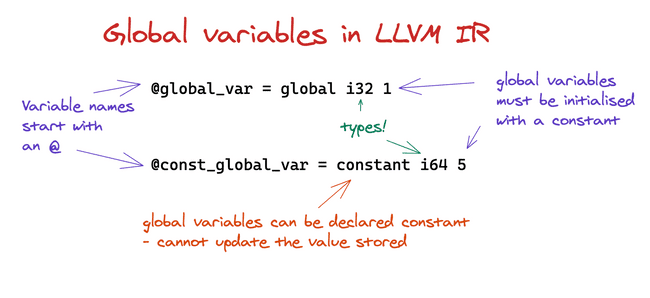
\includegraphics[width=\linewidth]{08_files/global-variables.png}} }

We can use the \texttt{module} object to create named global variables,
and to query them.

%Copy

\begin{verbatim}
module->getOrInsertGlobal(globalVarName, globalVarType);
...
GlobalVariable *globalVar = module->getNamedGlobal(globalVarName);
\end{verbatim}

Global variables \textbf{must} be initialised with a constant value (not
a variable):

%Copy

\begin{verbatim}
globalVar->setInitializer(initValue);
\end{verbatim}

Alternatively we can do this in one command using the
\texttt{GlobalVariable} constructor:

%Copy

\begin{lstlisting}[language=C++]
GlobalVariable *globalVar = new GlobalVariable(module, globalVarType, /*isConstant*/ false,              GlobalValue::ExternalLinkage, initValue, globalVarName)
\end{lstlisting}

As before we can \texttt{load} and \texttt{store}:

%Copy

\begin{verbatim}
builder->CreateLoad(globalVar);
builder->CreateStore(someVal, globalVar); // not for consts!
\end{verbatim}

\hypertarget{geps}{%
\section{\texorpdfstring{\protect\hyperlink{geps}{}GEPs}{GEPs}}\label{geps}}

We get a \textbf{base pointer} to the aggregate type (array / struct) on
the stack or in global memory, but what if we want a pointer to a
\textbf{specific element}? We'd need to find the \textbf{pointer offset}
of that element within the aggregate, and then add this to the base
pointer to get the address of that element. Calculating the pointer
offset is machine-specific e.g. depends on the size of the datatypes,
the struct padding etc.

The Get Element Pointer (GEP) instruction is an instruction to apply the
pointer offset to the base pointer and return the resultant
\textbf{pointer}.

Consider two arrays starting at \texttt{p}. Following C convention, we
can represent a pointer to that array as \texttt{char*} or
\texttt{int*}.

{
\href{https://mukulrathi.com/static/72077af5568512fb3538183382b672b0/a9577/pointer-offset.png}{{}
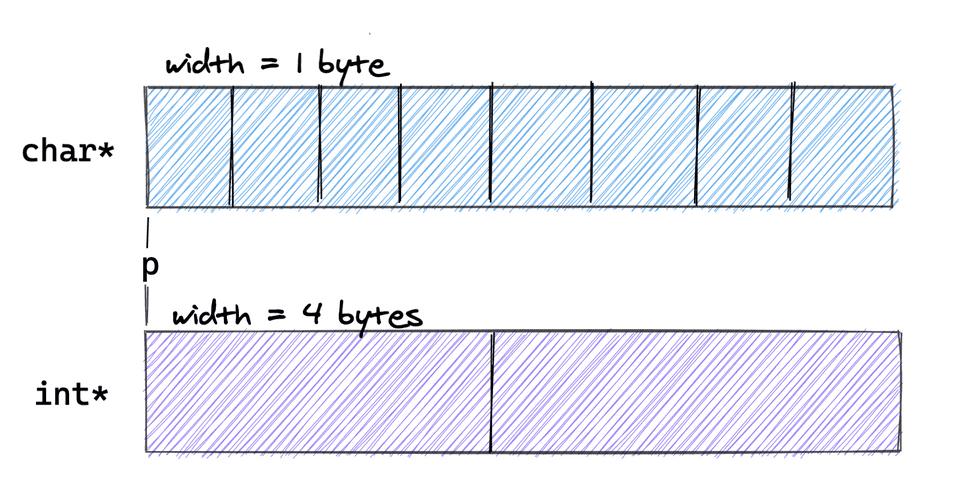
\includegraphics[width=\linewidth]{08_files/pointer-offset.png}} }

Below we show the GEP instruction to calculate the pointer \texttt{p+1}
in each of the arrays:

%Copy

\begin{lstlisting}[language=llvm]
// char = 8 bit integer = i8
%idx1 = getelementptr i8, i8* %p, i64 1 // p + 1 for char*
%idx2 = getelementptr i32, i32* %p, i64 1 // p + 1 for int*
\end{lstlisting}

This GEP instruction is a bit of a mouthful so here's a breakdown:

{
\href{https://mukulrathi.com/static/c54f577c6586b64d172044af4f8aacd1/79166/gep-int.png}{{}
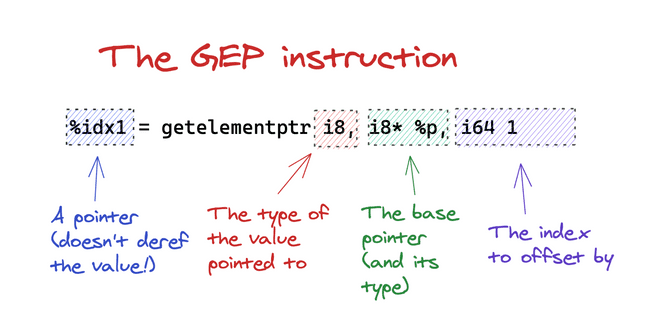
\includegraphics[width=\linewidth]{08_files/gep-int.png}} }

This \texttt{i64\ 1} index adds \textbf{multiples} of the base type to
the base pointer. \texttt{p+1} for \texttt{i8} would add 1 byte, whereas
as \texttt{p+1} for \texttt{i32} would add 4 bytes to \texttt{p}. If the
index was \texttt{i64\ 0} we'd return \texttt{p} itself.

The LLVM API instruction for creating a GEP is\ldots{}
\texttt{CreateGEP}.

%Copy

\begin{verbatim}
Value *ptr = builder->CreateGEP(baseType, basePtr, arrayofIndices);
\end{verbatim}

Wait? \emph{Array} of indices? Yes, the GEP instruction can have
multiple indices passed to it. We've looked at a simple example where we
only needed one index.

Before we look at the case where we pass multiple indices, I want to
reiterate the purpose of this first index:

\emph{\textbf{A pointer of type \texttt{Foo\ *} can represent in C the
base pointer of an array of type \texttt{Foo}. The first index adds
multiples of this base type Foo to traverse this array.}}

\hypertarget{geps-with-structs}{%
\subsection{\texorpdfstring{\protect\hyperlink{geps-with-structs}{}GEPS
with Structs}{GEPS with Structs}}\label{geps-with-structs}}

Okay, now let's look at structs. So take a struct of type \texttt{Foo}:

%Copy

\begin{lstlisting}[language=llvm]
%Foo = type { i32, [4 x i32], i32}
\end{lstlisting}

We want to index \textbf{specific} fields in the struct. The natural way
would be to label them field \texttt{0}, \texttt{1} and \texttt{2}. We
can access field \texttt{2} by passing this into the GEP instruction as
\textbf{another index}.

%Copy

\begin{lstlisting}[language=llvm]
%ThirdFieldPtr = getelementptr  %Foo, %Foo* %ptr, i64 0, i64 2
\end{lstlisting}

The returned pointer is then calculated as:
\texttt{ptr\ +\ 0\ *\ (size\ of\ Foo)\ +\ offset\ 2\ *\ (fields\ of\ Foo)}.

For structs, you'll likely always pass the first index as \texttt{0}.
The biggest confusion with GEPs is that this \texttt{0} can seem
redundant, as we want the field \texttt{2}, so why are we passing a
\texttt{0} index first? Hopefully you can see from the first example why
we need that \texttt{0}. Think of it as passing to GEP the base pointer
of an implicit \texttt{Foo} array of size 1.

To avoid the confusion, LLVM has a special \texttt{CreateStructGEP}
instruction that asks only for field index (this is the
\texttt{CreateGEP} instruction with a \texttt{0} added for you):

%Copy

\begin{verbatim}
Value *thirdFieldPtr = builder->CreateStructGEP(baseStructType, basePtr, fieldIndex);
\end{verbatim}

The more nested our aggregate structure, the more indices we can
provide. E.g. for element index \texttt{2} of Foo's second field (the 4
element int array):

%Copy

\begin{lstlisting}[language=llvm]
getelementptr  %Foo, %Foo* %ptr, i64 0, i64 1, i64 2
\end{lstlisting}

The pointer returned is:
\texttt{ptr\ +\ 0\ *\ (size\ of\ Foo)\ +\ offset\ 1\ *\ (field\ of\ Foo)\ +\ offset\ 2\ *\ (elems\ of\ array)}.
(In terms of the corresponding API, we'd use \texttt{CreateGEP} and pass
the array \texttt{\{0,1,2\}}.)
%\href{https://youtu.be/m8G_S5LwlTo?t=1753}
{A Good talk that explains GEP
well:\url{https://youtu.be/m8G_S5LwlTo?t=1753}}

\hypertarget{mem2reg}{%
\section{\texorpdfstring{\protect\hyperlink{mem2reg}{}mem2reg}{mem2reg}}\label{mem2reg}}

If you remember, LLVM IR must be written in SSA form. But what happens
if the Bolt source program we're trying to map to LLVM IR is not in SSA
form? For example, if we're reassigning \texttt{x}:

%{reassign\_var.bolt}

%Copy

\begin{verbatim}
let x = 1
x = x + 1
\end{verbatim}

One option would be for us to rewrite the program in SSA form in an
earlier compiler stage. Every time we reassign a variable, we'd have to
create a fresh variable. We'd also have to introduce \texttt{phi} nodes
for conditional statements. For our example, this is straightforward,
but in general this extra rewrite is a pain we would rather not deal
with.

%{assign\_fresh\_vars.bolt}

%Copy

\begin{verbatim}
// Valid SSA: assign fresh variables
let x1 = 1
    x2 = x1 + 1
\end{verbatim}

We can use \textbf{pointers} to avoid assigning fresh variables. Note
here we \textbf{aren't reassigning} the pointer \texttt{x}, just
updating \textbf{the value it pointed to}. So this is valid SSA.

%Copy

\begin{verbatim}
// valid SSA: use a pointer and update the value it points to
let x = &1;
   *x = *x + 1
\end{verbatim}

This switch to pointers is a much easier transformation than variable
renaming. It also has a really nice LLVM IR equivalent: allocating
\emph{stack memory} (and manipulating the pointers to the stack) instead
of reading from \emph{registers}.

So whenever we declare a local variable, we use \texttt{alloca} to get a
pointer to freshly allocated stack space. We use the \texttt{load} and
\texttt{store} instructions to read and update the value pointed to by
the pointer:

%{reassign\_var.ll}
%
%Copy

\begin{lstlisting}[language=llvm]
%x = alloca i32
store i32 1, i32* %x

%1 = load i32, i32* %x
%2 = add i32 %1, 1
store i32 %2, i32* %x
\end{lstlisting}

Let's revisit the LLVM IR if we were to rewrite the Bolt program to use
fresh variables. It's only \emph{2} instructions, compared to the
\emph{5} instructions needed if using the stack. Moreover, we avoid the
expensive \texttt{load} and \texttt{store} memory access instructions.

%{assign\_fresh\_vars.ll}
%
%Copy

\begin{lstlisting}[language=llvm]
%x1 = 1
%x2 = add i32 %x1, 1   // let x2 = x1 + 1
\end{lstlisting}

So while we've made our lives easier as compiler writers by avoiding a
rewrite-to-SSA pass, this has come at the expense of performance.

Happily, LLVM lets us have our cake and eat it.

LLVM provides a \texttt{mem2reg} optimisation that optimises stack
memory accesses into register accesses. We just need to ensure we
declare all our \texttt{alloca}s for local variables in the
\textbf{entry basic block} for the function.

How do we do this if the local variable declaration occurs midway
through the function, in another block? Let's look at an example:

%Copy

\begin{verbatim}
// BOLT variable declaration
let x : int = someVal;
// translated to LLVM IR
%x = alloca i32
store i32 someVal, i32* %x
\end{verbatim}

We can actually move the \texttt{alloca}. It doesn't matter where we
allocate the stack space so long as it is allocated before use. So let's
write the \texttt{alloca} at the very start of the parent function this
local variable declaration occurs.

How do we do this in the API? Well, remember the analogy of the builder
being like a file pointer? We can have multiple file pointers pointing
to different places in the file. Likewise, we instantiate a new
\texttt{IRBuilder} to point to the start of the \texttt{entry} basic
block of the parent function, and insert the \texttt{alloca}
instructions using that builder.

%{
%\href{https://github.com/mukul-rathi/bolt/blob/master/src/llvm-backend/llvm_ir_codegen/expr_codegen.cc\#L127-L131}{expr\_codegen.cc}}
%
%Copy

\begin{lstlisting}[language=C++,caption={expr\_codegen.cc}]
Function *parentFunction = builder->GetInsertBlock()
                                ->getParent();
// create temp builder to point to start of function
IRBuilder<> TmpBuilder(&(parentFunction->getEntryBlock()),
                        parentFunction->getEntryBlock().begin());
// .begin() inserts this alloca at beginning of block
AllocaInst *var = TmpBuilder.CreateAlloca(boundVal->getType());
// resume our current position by using orig. builder
builder->CreateStore(someVal, var);
\end{lstlisting}

%\hypertarget{i-make-content-about-my-software-engineering-journey-curated-in-my-newsletter}{%
%\subsection{I make content about my software engineering journey,
%curated in my
%newsletter!}\label{i-make-content-about-my-software-engineering-journey-curated-in-my-newsletter}}
%
%Tips from my time at Cambridge and Facebook, and early access to
%technical tutorials on machine learning, compilers and beyond.
%
%\href{https://newsletter.mukulrathi.com/}{Check out previous issues!}
%
%Email Address
%
%By subscribing, you agree with Revue's
%\href{https://www.getrevue.co/terms}{Terms of Service} and
%\href{https://www.getrevue.co/privacy}{Privacy Policy}.
%
%\hypertarget{llvm-optimisations}{%
%\section{\texorpdfstring{\protect\hyperlink{llvm-optimisations}{}LLVM
%Optimisations}{LLVM Optimisations}}\label{llvm-optimisations}}
%
%The API makes it really easy to add passes. We create a
%\texttt{functionPassManager}, add the optimisation passes we'd like, and
%then initialise the manager.

%{
%\href{https://github.com/mukul-rathi/bolt/blob/master/src/llvm-backend/llvm_ir_codegen/ir_codegen_visitor.cc\#L68-L83}{ir\_codegen\_visitor.cc}}
%
%Copy

\begin{lstlisting}[caption={ir\_codegen\_visitor.cc},language=C++]
std::unique_ptr<legacy::FunctionPassManager> functionPassManager =
      make_unique<legacy::FunctionPassManager>(module.get());

  // Promote allocas to registers.
  functionPassManager->add(createPromoteMemoryToRegisterPass());
  // Do simple "peephole" optimizations
  functionPassManager->add(createInstructionCombiningPass());
  // Reassociate expressions.
  functionPassManager->add(createReassociatePass());
  // Eliminate Common SubExpressions.
  functionPassManager->add(createGVNPass());
  // Simplify the control flow graph (deleting unreachable blocks etc).
  functionPassManager->add(createCFGSimplificationPass());

  functionPassManager->doInitialization();
\end{lstlisting}

We run this on each of the program's functions:

%{
%\href{https://github.com/mukul-rathi/bolt/blob/master/src/llvm-backend/llvm_ir_codegen/ir_codegen_visitor.cc\#L68-L83}{ir\_codegen\_visitor.cc}}
%
%Copy

\begin{lstlisting}[language=C++,caption={ir\_codegen\_visitor.cc}]
for (auto &function : functions) {
    Function *llvmFun =
     module->getFunction(StringRef(function->functionName));
    functionPassManager->run(*llvmFun);
  }
  Function *llvmMainFun = module->getFunction(StringRef("main"));
  functionPassManager->run(*llvmMainFun);
\end{lstlisting}

In particular, let's look at the the \texttt{factorial} LLVM IR output
by our Bolt compiler before and after. You can find them in the repo:

%{
%\href{https://github.com/mukul-rathi/bolt/blob/master/examples/factorial-unoptimised.ll}{factorial-unoptimised.ll}}
%
%Copy

\begin{lstlisting}[language=llvm,caption={{factorial-unoptimised.ll}}]
define i32 @factorial(i32) {
entry:
  %n = alloca i32
  store i32 %0, i32* %n
  %1 = load i32, i32* %n
  %eq = icmp eq i32 %1, 0
  br i1 %eq, label %then, label %else

then:                                             ; preds = %entry
  br label %ifcont

else:                            ; preds = %entry
  %2 = load i32, i32* %n
  %3 = load i32, i32* %n
  %sub = sub i32 %3, 1
  %4 = call i32 @factorial(i32 %sub)
  %mult = mul i32 %2, %4
  br label %ifcont

ifcont:                     ; preds = %else, %then
  %iftmp = phi i32 [ 1, %then ], [ %mult, %else ]
  ret i32 %iftmp
}
\end{lstlisting}

And the optimised version:

%{
%\href{https://github.com/mukul-rathi/bolt/blob/master/examples/factorial-optimised.ll}{factorial-optimised.ll}}
%
%Copy

\begin{lstlisting}[language=llvm,caption={{factorial-optimised.ll}}]
define i32 @factorial(i32) {
entry:
  %eq = icmp eq i32 %0, 0
  br i1 %eq, label %ifcont, label %else

else:                                             ; preds = %entry
  %sub = add i32 %0, -1
  %1 = call i32 @factorial(i32 %sub)
  %mult = mul i32 %1, %0
  br label %ifcont

ifcont:                                           ; preds = %entry, %else
  %iftmp = phi i32 [ %mult, %else ], [ 1, %entry ]
  ret i32 %iftmp
}
\end{lstlisting}

Notice how we've actually got rid of the \texttt{alloca} and the
associated \texttt{load} and \texttt{store} instructions, and also
removed the \texttt{then} basic block!

\hypertarget{wrap-up}{%
\section{\texorpdfstring{\protect\hyperlink{wrap-up}{}Wrap
up}{Wrap up}}\label{wrap-up}}

This last example shows you the power of LLVM and its optimisations. You
can find the top-level code that runs the LLVM code generation and
optimisation in the
\href{https://github.com/mukul-rathi/bolt/blob/master/src/llvm-backend/main.cc}{main.cc}
file in the Bolt repository.

In the next few posts we'll be looked at some more advanced language
features: generics, inheritance and method overriding and concurrency!
Stay tuned for when they come out!

%\hypertarget{share-this-on-twitter}{%
%\subsection{Share This On Twitter}\label{share-this-on-twitter}}
%
%If you liked this post, please consider sharing it with your network. If
%you have any questions, tweet away and I'll answer :) I also tweet when
%new posts drop!
%
%\textbf{PS:} I also share helpful tips and links as I'm learning - so
%you get them \textbf{well before} they make their way into a post!
%
%\hypertarget{series-creating-the-bolt-compiler-1}{%
%\section{Series: Creating the Bolt
%Compiler}\label{series-creating-the-bolt-compiler-1}}
%
%\begin{itemize}
%\item
%  { Part 1:
%  }\href{https://mukulrathi.com/create-your-own-programming-language/intro-to-compiler/}{How
%  I wrote my own "proper" programming language}
%\item
%  { Part 2:
%  }\href{https://mukulrathi.com/create-your-own-programming-language/compiler-engineering-structure/}{So
%  how do you structure a compiler project?}
%\item
%  { Part 3:
%  }\href{https://mukulrathi.com/create-your-own-programming-language/parsing-ocamllex-menhir/}{Writing
%  a Lexer and Parser using OCamllex and Menhir}
%\item
%  { Part 4:
%  }\href{https://mukulrathi.com/create-your-own-programming-language/intro-to-type-checking/}{An
%  accessible introduction to type theory and implementing a
%  type-checker}
%\item
%  { Part 5:
%  }\href{https://mukulrathi.com/create-your-own-programming-language/data-race-dataflow-analysis/}{A
%  tutorial on liveness and alias dataflow analysis}
%\item
%  { Part 6:
%  }\href{https://mukulrathi.com/create-your-own-programming-language/lower-language-constructs-to-llvm/}{Desugaring
%  - taking our high-level language and simplifying it!}
%\item
%  { Part 7:
%  }\href{https://mukulrathi.com/create-your-own-programming-language/protobuf-ocaml-cpp-tutorial/}{A
%  Protobuf tutorial for OCaml and C++}
%\item
%  \textbf{Part 8: A Complete Guide to LLVM for Programming Language
%  Creators}
%\item
%  { Part 9:
%  }\href{https://mukulrathi.com/create-your-own-programming-language/concurrency-runtime-language-tutorial/}{Implementing
%  Concurrency and our Runtime Library}
%\item
%  { Part 10:
%  }\href{https://mukulrathi.com/create-your-own-programming-language/generics-parametric-polymorphism/}{Generics
%  - adding polymorphism to Bolt}
%\item
%  { Part 11:
%  }\href{https://mukulrathi.com/create-your-own-programming-language/inheritance-method-overriding-vtable/}{Adding
%  Inheritance and Method Overriding to Our Language}
%\end{itemize}
%
%\begin{itemize}
%\item ~
%  \hypertarget{how-do-i-use__-a-guide-to-react-hooks}{%
%  \subsection{\texorpdfstring{\href{https://mukulrathi.com/intro-to-react/react-hooks-complete-guide/}{←
%  How do I use\_\_? A guide to React
%  hooks}}{← How do I use\_\_? A guide to React hooks}}\label{how-do-i-use__-a-guide-to-react-hooks}}
%\item ~
%  \hypertarget{implementing-concurrency-and-our-runtime-library}{%
%  \subsection{\texorpdfstring{\href{https://mukulrathi.com/create-your-own-programming-language/concurrency-runtime-language-tutorial/}{Implementing
%  Concurrency and our Runtime Library
%  →}}{Implementing Concurrency and our Runtime Library →}}\label{implementing-concurrency-and-our-runtime-library}}
%\end{itemize}
%
%\hypertarget{table-of-contents}{%
%\section{Table of Contents}\label{table-of-contents}}
%
%\href{https://mukulrathi.com/create-your-own-programming-language/llvm-ir-cpp-api-tutorial/\#top-of-page}{}
%
%\hypertarget{a-complete-guide-to-llvm-for-programming-language-creators}{%
%\subsection{A Complete Guide to LLVM for Programming Language
%Creators}\label{a-complete-guide-to-llvm-for-programming-language-creators}}
%
%\begin{itemize}
%\item
%  \href{https://mukulrathi.com/create-your-own-programming-language/llvm-ir-cpp-api-tutorial/\#whos-this-tutorial-for}{}
%
%  \hypertarget{whos-this-tutorial-for-1}{%
%  \subsection{Who's this tutorial
%  for?}\label{whos-this-tutorial-for-1}}
%\item
%  \href{https://mukulrathi.com/create-your-own-programming-language/llvm-ir-cpp-api-tutorial/\#just-give-me-the-code}{}
%
%  \hypertarget{just-give-me-the-code-1}{%
%  \subsection{Just give me the code!}\label{just-give-me-the-code-1}}
%\item
%  \href{https://mukulrathi.com/create-your-own-programming-language/llvm-ir-cpp-api-tutorial/\#understanding-llvm-ir}{}
%
%  \hypertarget{understanding-llvm-ir-1}{%
%  \subsection{Understanding LLVM IR}\label{understanding-llvm-ir-1}}
%
%  \begin{itemize}
%  \item
%    \href{https://mukulrathi.com/create-your-own-programming-language/llvm-ir-cpp-api-tutorial/\#an-example-factorial}{}
%
%    \hypertarget{an-example-factorial-1}{%
%    \subsection{An example: Factorial}\label{an-example-factorial-1}}
%  \end{itemize}
%\item
%  \href{https://mukulrathi.com/create-your-own-programming-language/llvm-ir-cpp-api-tutorial/\#the-llvm-api-key-concepts}{}
%
%  \hypertarget{the-llvm-api-key-concepts-1}{%
%  \subsection{The LLVM API: Key
%  Concepts}\label{the-llvm-api-key-concepts-1}}
%
%  \begin{itemize}
%  \item
%    \href{https://mukulrathi.com/create-your-own-programming-language/llvm-ir-cpp-api-tutorial/\#irbuilder}{}
%
%    \hypertarget{irbuilder-1}{%
%    \subsection{IRBuilder}\label{irbuilder-1}}
%  \item
%    \href{https://mukulrathi.com/create-your-own-programming-language/llvm-ir-cpp-api-tutorial/\#types-and-constants}{}
%
%    \hypertarget{types-and-constants-1}{%
%    \subsection{Types and Constants}\label{types-and-constants-1}}
%  \item
%    \href{https://mukulrathi.com/create-your-own-programming-language/llvm-ir-cpp-api-tutorial/\#type-declarations}{}
%
%    \hypertarget{type-declarations-1}{%
%    \subsection{Type declarations}\label{type-declarations-1}}
%  \end{itemize}
%\item
%  \href{https://mukulrathi.com/create-your-own-programming-language/llvm-ir-cpp-api-tutorial/\#more-llvm-ir-concepts}{}
%
%  \hypertarget{more-llvm-ir-concepts-1}{%
%  \subsection{More LLVM IR Concepts}\label{more-llvm-ir-concepts-1}}
%\item
%  \href{https://mukulrathi.com/create-your-own-programming-language/llvm-ir-cpp-api-tutorial/\#stack-allocation}{}
%
%  \hypertarget{stack-allocation-1}{%
%  \subsection{Stack allocation}\label{stack-allocation-1}}
%\item
%  \href{https://mukulrathi.com/create-your-own-programming-language/llvm-ir-cpp-api-tutorial/\#global-variables}{}
%
%  \hypertarget{global-variables-1}{%
%  \subsection{Global variables}\label{global-variables-1}}
%\item
%  \href{https://mukulrathi.com/create-your-own-programming-language/llvm-ir-cpp-api-tutorial/\#geps}{}
%
%  \hypertarget{geps-1}{%
%  \subsection{GEPs}\label{geps-1}}
%
%  \begin{itemize}
%  \item
%    \href{https://mukulrathi.com/create-your-own-programming-language/llvm-ir-cpp-api-tutorial/\#geps-with-structs}{}
%
%    \hypertarget{geps-with-structs-1}{%
%    \subsection{GEPS with Structs}\label{geps-with-structs-1}}
%  \end{itemize}
%\item
%  \href{https://mukulrathi.com/create-your-own-programming-language/llvm-ir-cpp-api-tutorial/\#mem2reg}{}
%
%  \hypertarget{mem2reg-1}{%
%  \subsection{mem2reg}\label{mem2reg-1}}
%\item
%  \href{https://mukulrathi.com/create-your-own-programming-language/llvm-ir-cpp-api-tutorial/\#llvm-optimisations}{}
%
%  \hypertarget{llvm-optimisations-1}{%
%  \subsection{LLVM Optimisations}\label{llvm-optimisations-1}}
%\item
%  \href{https://mukulrathi.com/create-your-own-programming-language/llvm-ir-cpp-api-tutorial/\#wrap-up}{}
%
%  \hypertarget{wrap-up-1}{%
%  \subsection{Wrap up}\label{wrap-up-1}}
%\end{itemize}
%
%© Mukul Rathi 2023
%
%\hypertarget{gatsby-announcer}{}
%Navigated to A Complete Guide to LLVM for Programming Language Creators
